\chapter{Analysis}\label{chap:analysis}

The data recorded by the oscilloscopes, in the form of waveforms, was pre-processed using the software PyAna~\cite{atlas_hgtd_pyana_2025}. Another software, PaTrack~\cite{atlas_hgtd_patrack_2025}, used the spacial information from the MIMOSA planes to reconstruct the tracks of the particles. The data was then combined into ROOT files to be further analyzed.

Some quality cuts were applied to the data, to remove extra noise. To illustrate the analysis procedure that was followed in this study, a single DUT was picked as an example. All the plots in this chapter (unless otherwise stated) refer to the sensor IMEv3-W12, a 2\(\times\)2 array of LGADs, operated at \qty{-30}{\degreeCelsius} and perpendicular to the beam.

\section{Data pre-processing}

The pre-processing was performed by other collaborators prior to this analysis. The steps of the pre-processing are described below.

\begin{figure}[h!btp]
    \centering
    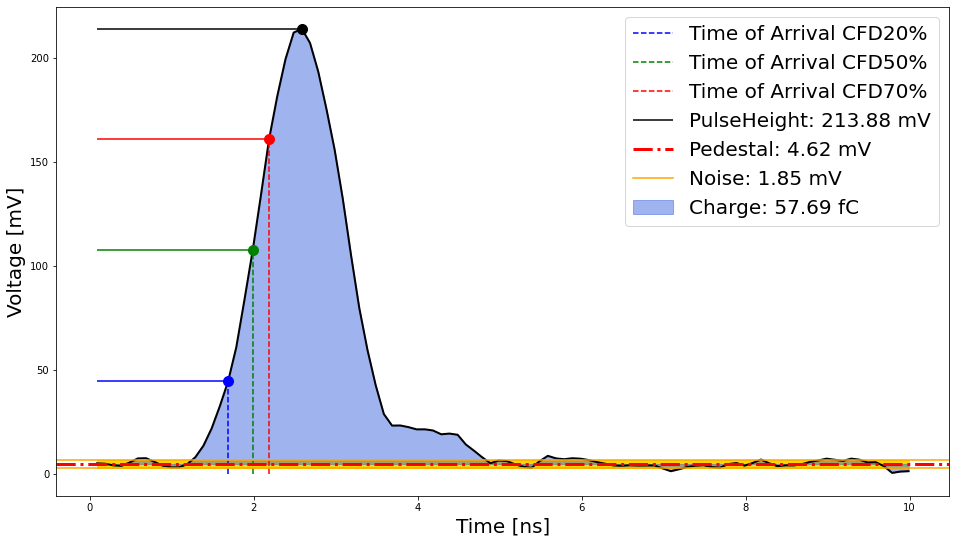
\includegraphics[width=1\linewidth]{Images/methods/Waveform of particle, channel2, with CFD (ns).png}
    \captionsetup{width=\captionwidth}
    \caption{An example of a pulse with its main features highlighted. The pedestal (red dotted line) is the mean of the background signals, the noise (yellow) is its standard deviation, the pulse height (black) is the maximum amplitude and the charge (light blue) is the area under the pulse. The remaining three dashed lines (blue, green and red) correspond to the TOA associated to three different values of CFD (20\%, 50\% and 70\%, respectively).}
    \label{fig:waveform_features}
\end{figure} 

%PyAna, aka pulse description
Whenever a trigger was detected, the oscilloscopes recorded an event. For each event, at least 2000 samples were collected, spaced every \qty{25}{\pico\second}, an example of one event (a pulse) is shown in Figure~\ref{fig:waveform_features}. This pulse (waveform) was then processed with PyAna.

Firstly, the pedestal and the noise were measured by computing the mean and standard deviation, respectively, using the first 240 samples, where no signal is expected \cite{Allaire:2018bof}. Secondly, the maximum of the pulse was found by a second-degree polynomial fit, in a \qty{400}{\pico\second} window around the sample with the highest amplitude. After subtracting the pedestal, the total charge was computed as the integral of the pulse divided by the transimpedance\footnote{Transfer impedance, it is the ratio of output voltage to input current in the readout board, expressed in \unit{\ohm}} value of the board the LGAD is mounted on (Equation~\ref{eq:charge_integral}). The integral is computed in a window wide enough to contain the full pulse.

\begin{equation}\label{eq:charge_integral}
    Q = \frac{\int_{t_1}^{t_2} V(t)dt}{R_b} \, .
\end{equation}
Where \(Q\) is the charge, \(V\) is the voltage (as a function of time \(t\)), \(R_b\) is the transimpedance and \(t_2-t_1\) is the integration window.

%%% PaTrack, aka MIMOSA plane
The spacial information was processed with the PaTrack software to create tracks of the particles. Two straight tracklets, an "upstream" and a "downstream" tracklet passing through MIMOSA planes 1,2,3 and 4,5,6, respectively, were reconstructed to best fit the hits on each plane and meet at the longitudinal (z) location of the DUTs, Figure~\ref{fig:mimosa_tracking}. This provided each event with the XY intersection of the track onto the plane of each DUT. 

\begin{figure}[h!btp]
    \centering
    \includegraphics[width=1\linewidth]{Images/methods/MIMOSA tracking scheme.png}
    \captionsetup{width=\captionwidth}
    \caption{Scheme of the reconstructed tracks, made of two tracklets, one upstream and one upstream, as they best fit the hits on the MIMOSA planes before and after the DUTs.}
    \label{fig:mimosa_tracking}
\end{figure} 


To measure the time resolution it is crucial to define the Time of Arrival (TOA), i.e. the time at which the particle hits the sensor and the pulse is recorded. There are several ways to make this choice, including: Constant Threshold Discriminator (CTD), Constant Fraction Discriminator (CFD) and Zero Crossing Detector (ZCD), Figure~\ref{fig:constant fraction}.

In this study we chose to use the Constant Fraction Discriminator. More specifically, for the MCP a value of 50\% CFD was chosen, while for the DUTs a value of 20\% was chosen in all cases except for heavily irradiated sensors, in which 70\% yielded improved results overall. (An example of each in Figures~\ref{fig:CFD_comparison_unirradiated}~and~\ref{fig:CFD_comparison_irradiated}.)

\FloatBarrier

\section{Quality cuts}\label{sec:qualtiy_cuts}

% To remove the various sources of noise some quality cuts were applied to the data. %; in this section we explain these choices.
To ensure that only physically meaningful events were used in the measurements, it was necessary to apply some quality cuts to the initial data. These cuts were designed to reject events affected by various sources of noise or not meaningful to the analysis. 

To begin with, we removed events with low signal peak (or high noise). Subsequently, we used the pulse height information to identify the outline of each pad and select only events passing through it. Finally, we established a time window around the peak of the distribution to avoid negative effects caused by the neighbouring pads and the edges of the sensors (outside the gain layer).

\subsection{Noise cut}\label{subsec:noise_cut}
The most straightforward trimming consisted in the exclusion of signals which had a pulse height less than 3 times greater than the noise:

\begin{equation*}
    P > b + 3\sigma \, .
\end{equation*}

Where \(P\) is the maximum of the pulse (pulse height), \(b\) is pedestal baseline and \(\sigma\) is the noise. Since the noise is approximately normally distributed, applying this cut ensured that events arising from noise fluctuations were excluded with high confidence.

\subsection{Pulse height cut}\label{subsec:pulseHeight_cut}

% I think I want to cut out the title
\begin{figure}[h!tbp]
    \centering
    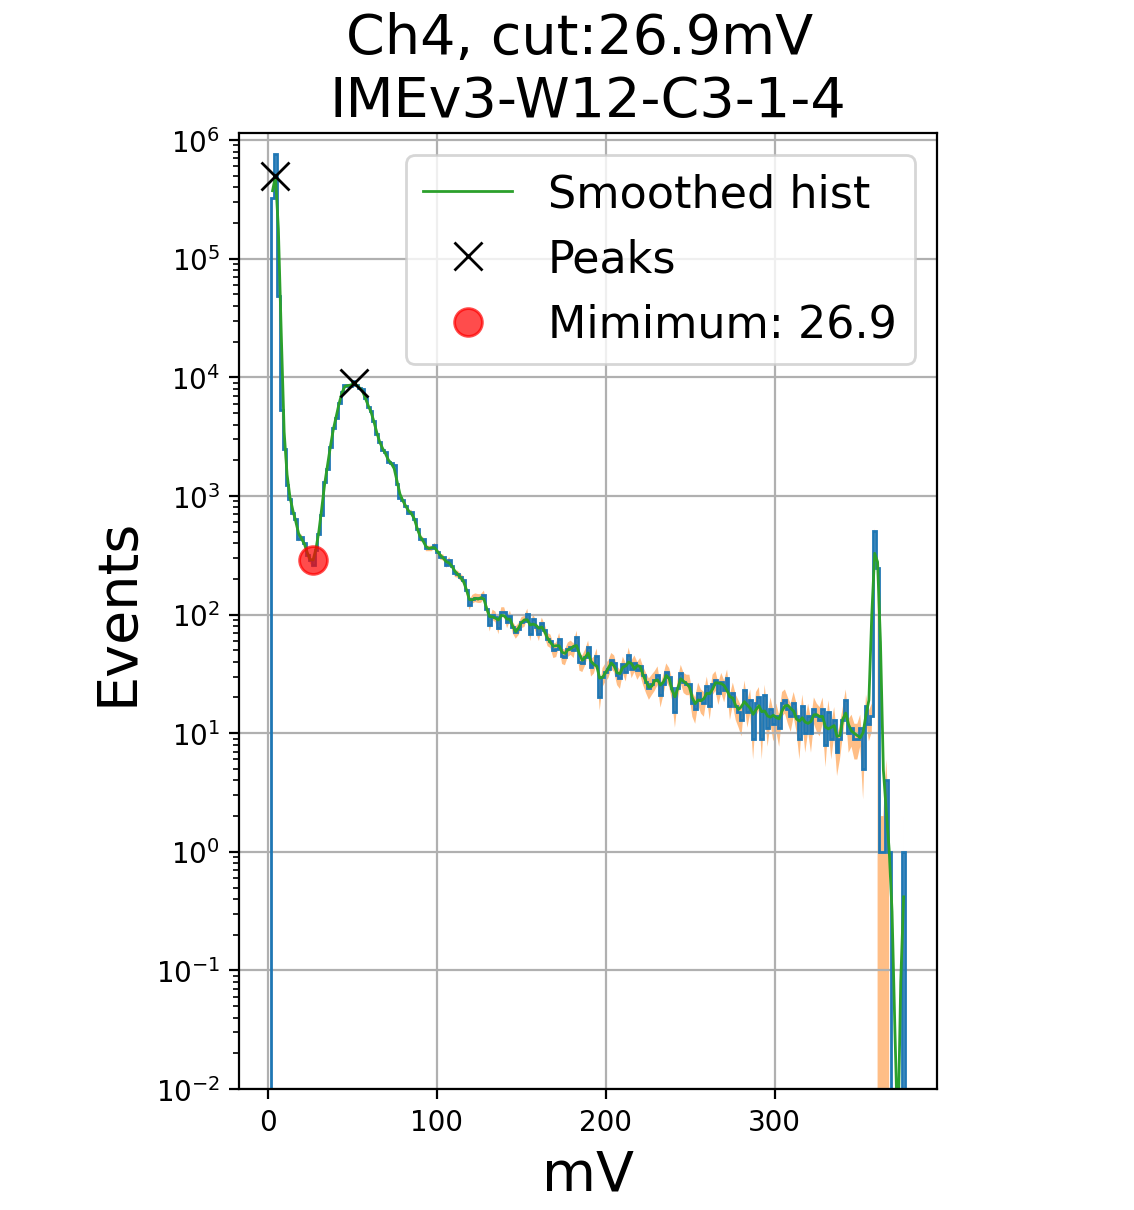
\includegraphics[width=.5\linewidth]{Images/methods/2D_Sensors_401 S1 pulseHeight cut_pulse.png}
    \captionsetup{width=\captionwidth}
    \caption{The pulse height cut was defined by the position of the local minimum between the two main peaks (identified as noise and signal). The rightmost spike of events was caused by some erroneous oscilloscope settings, explained in Section~\ref{sec:pulse_clipping}.}
    \label{fig:pulseHeight_cut}
\end{figure}

By plotting the distribution of pulse height values, we applied a cut to the pulses located below the local minimum in the distribution\footnote{A Kernel Density Estimator was used in order to smooth the distribution before identifying the minimum}, to separate guaranteed signals from potential noise. The goal of this cut was to select only events that were detected by the DUT, and use this information to find the physical outline of the pad.

Using this selection of events, the X and Y coordinates of the tracks were plotted, giving the result shown in Figure~\ref{fig:pulseHeight_cut_highlight}. The outline of the sensor is distinctly shown, making possible the subsequent quality cut: the selection of tracks that passed through the surface of the pad, i.e. a \textit{geometry cut}

\subsection{Geometry cut}\label{sec:geometry_cut}

\begin{figure}[h!tbp]
    \centering
    % \includesvg[width=1\linewidth]{Images/methods/locating_edges_Xtr_batch_401_S1_DUT3}
    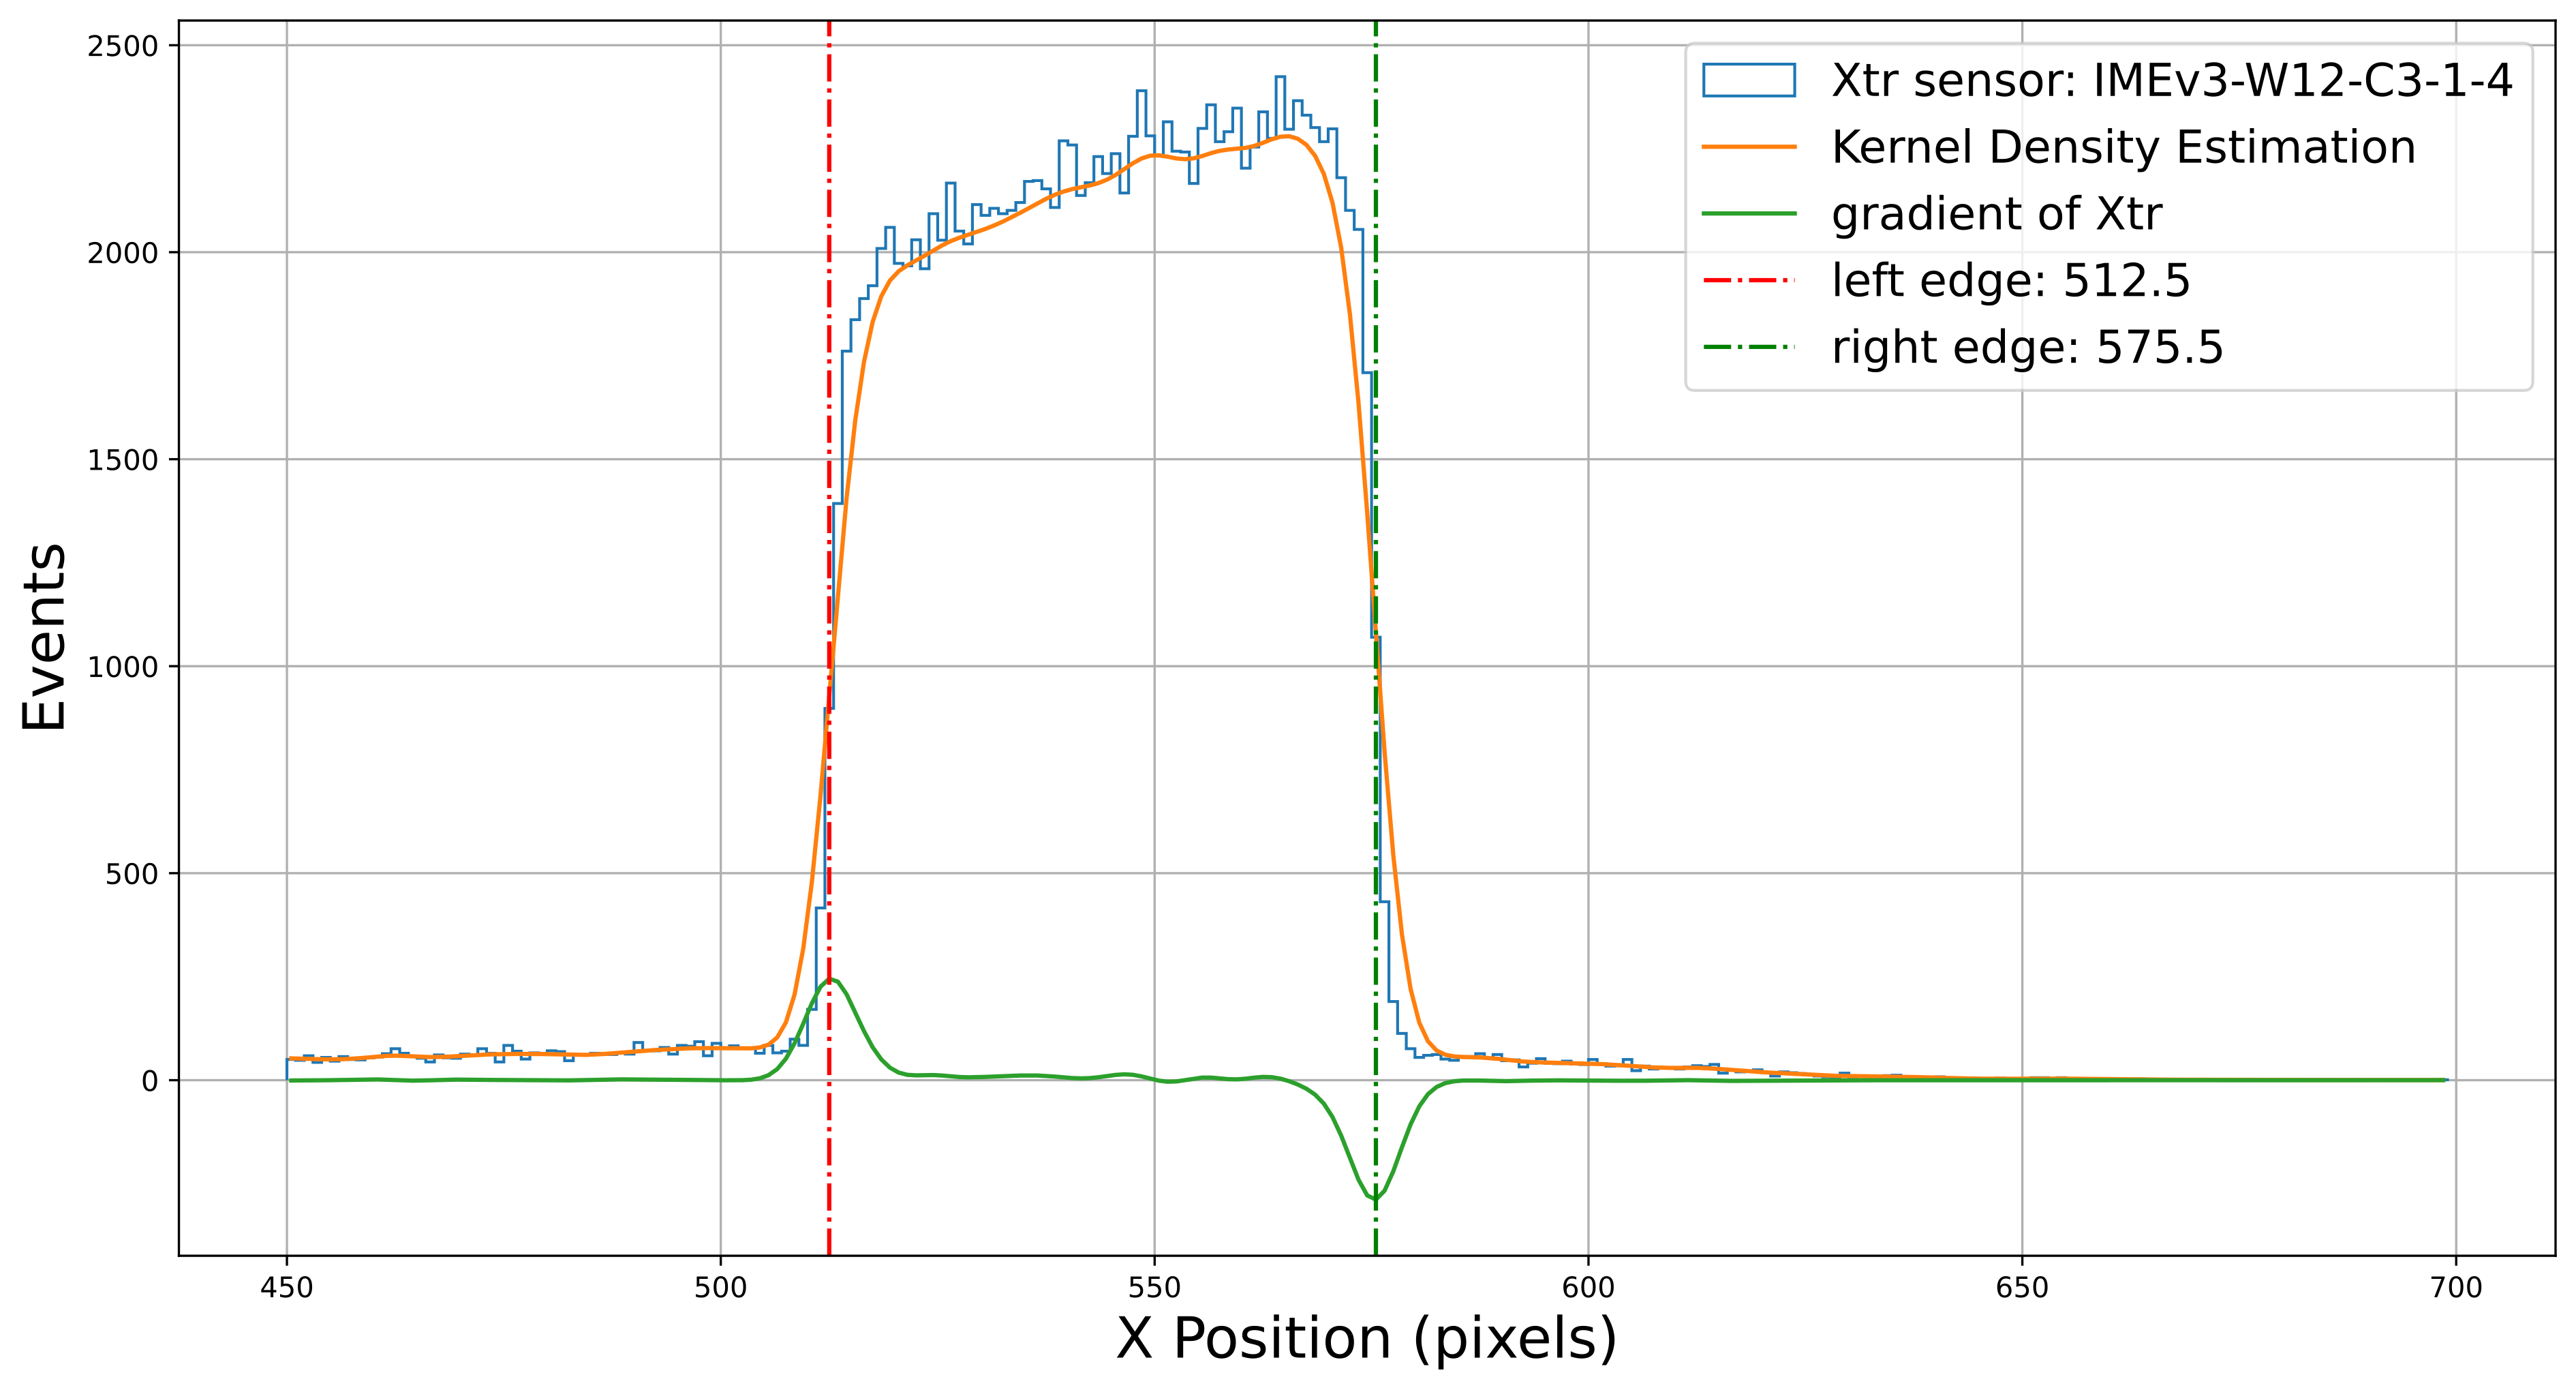
\includegraphics[width=.7\linewidth]{Images/methods/locating_edges_Xtr_batch_401_S1_DUT3.png}
    \captionsetup{width=\captionwidth}
    \caption{Projection of hits on the X axis after the \nameref{subsec:pulseHeight_cut}. By taking its derivative, it was possible to determine the position of the edges of the sensor. The unit is pixels of MIMOSA planes.}
    \label{fig:edges_of_the_sensor}
\end{figure}

Looking at the projections of hits on the X and Y coordinates, it was possible to determine the outline of the pad. The distribution was smoothed\footnote{Using a Kernel Density Estimator, as done previously for the pulse height distribution.} and its gradient (derivative) was calculated. This gave rise to two remarkably pronounced peaks shown in Figure~\ref{fig:edges_of_the_sensor}, which could be interpreted as the edges of the pads. By applying this procedure to both the X and Y projections we determined the horizontal and vertical edges, respectively. The final rectangular shape can be seen in Figure~\ref{fig:pulseHeight_cut_highlight}, alongside with the density of hits after applying a \textit{pulse height cut}. In few cases the sensors were slightly tilted in the XY plane, giving rise to slightly imprecise outlines, this is shown in \ref{fig:tilted_sensors}, although it did not have a significant impact on the rest of the analysis.

% NOTE: the edges defined like this are smaller than the real size of the pad (which is 1.3x1.3 mm\(^2\)) \cite{Agapopoulou_2022} \marginpar{\flushleft There is an outer guard ring isolating, so maybe the size is correct}

For certain properties that were analyzed (such as efficiency and time resolution) it became clear that the rough selection of the contour of the pad was not always sufficient. Thus, an additional \textit{central area cut} was set up. A region of \(0.5\times0.5\unit{\milli\meter^2}\) in the center of the pad was selected (similarly to what had been done in \cite{Agapopoulou_2022}) in order to avoid undesirable effects originating from the region outside the gain layer of the LGAD.

\begin{figure}[h!tbp]
    \centering
    \subfloat[The heatmap of the reconstructed tracks without any cuts applied. The large rectangular shape is produced by the region of interest (ROI) selected with the FE-I4.]{
        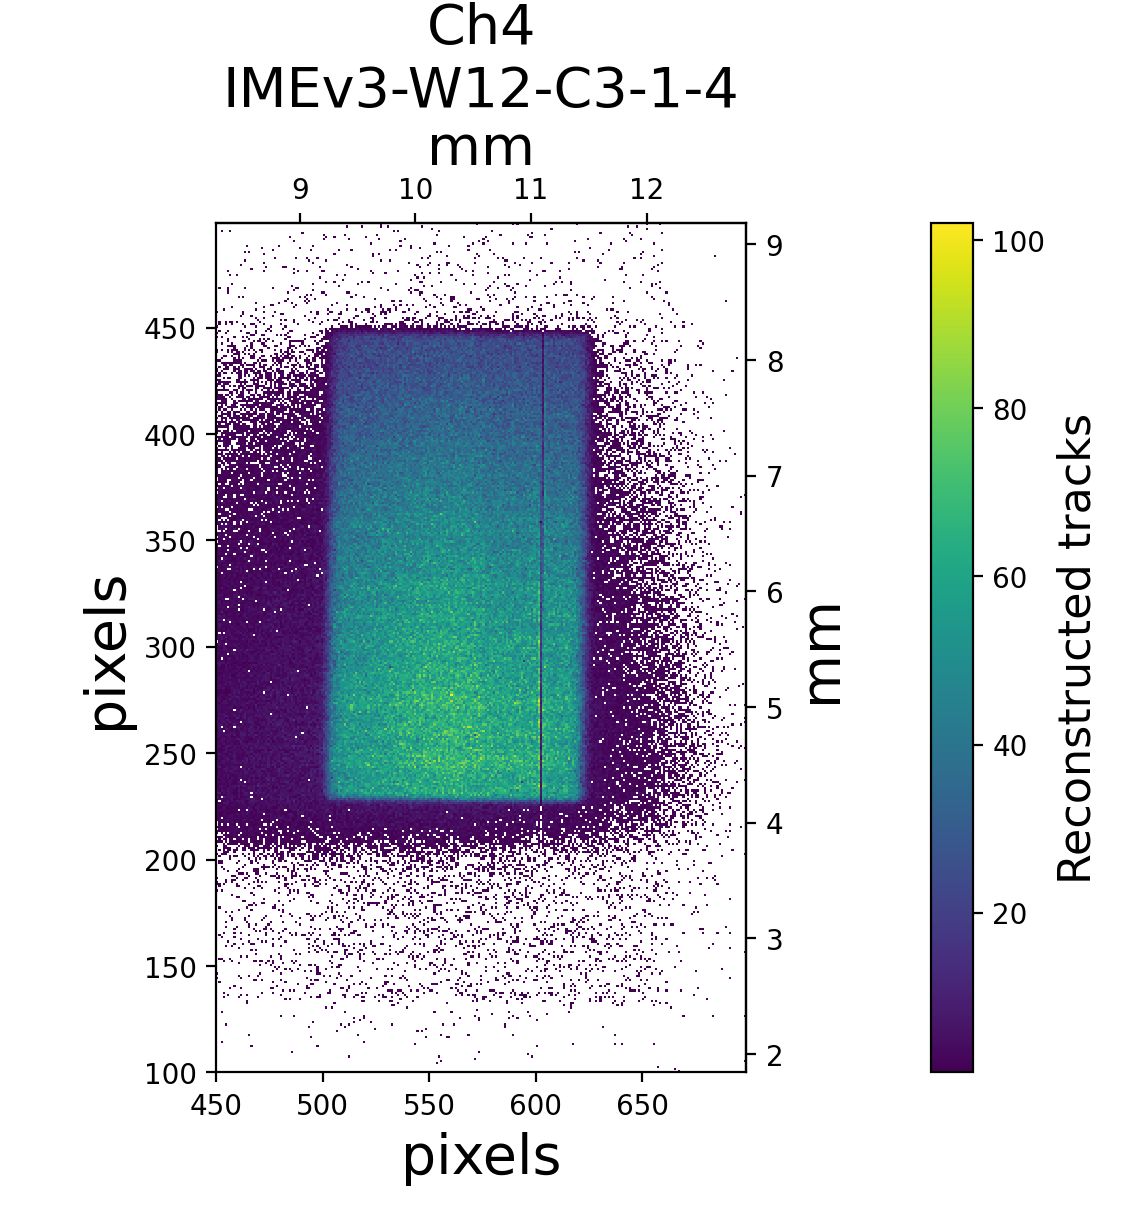
\includegraphics[width=.47\linewidth]{Images/methods/2D_Tracks_401 S1 (no cuts)_DUTs_3.png}
        \label{fig:hits_no_cuts}}
    \hfill
    \subfloat[The smaller rectangle corresponds to the area of the pad (highlighted in red with sides lengths) found by applying a \textit{pulse height cut}.]{
        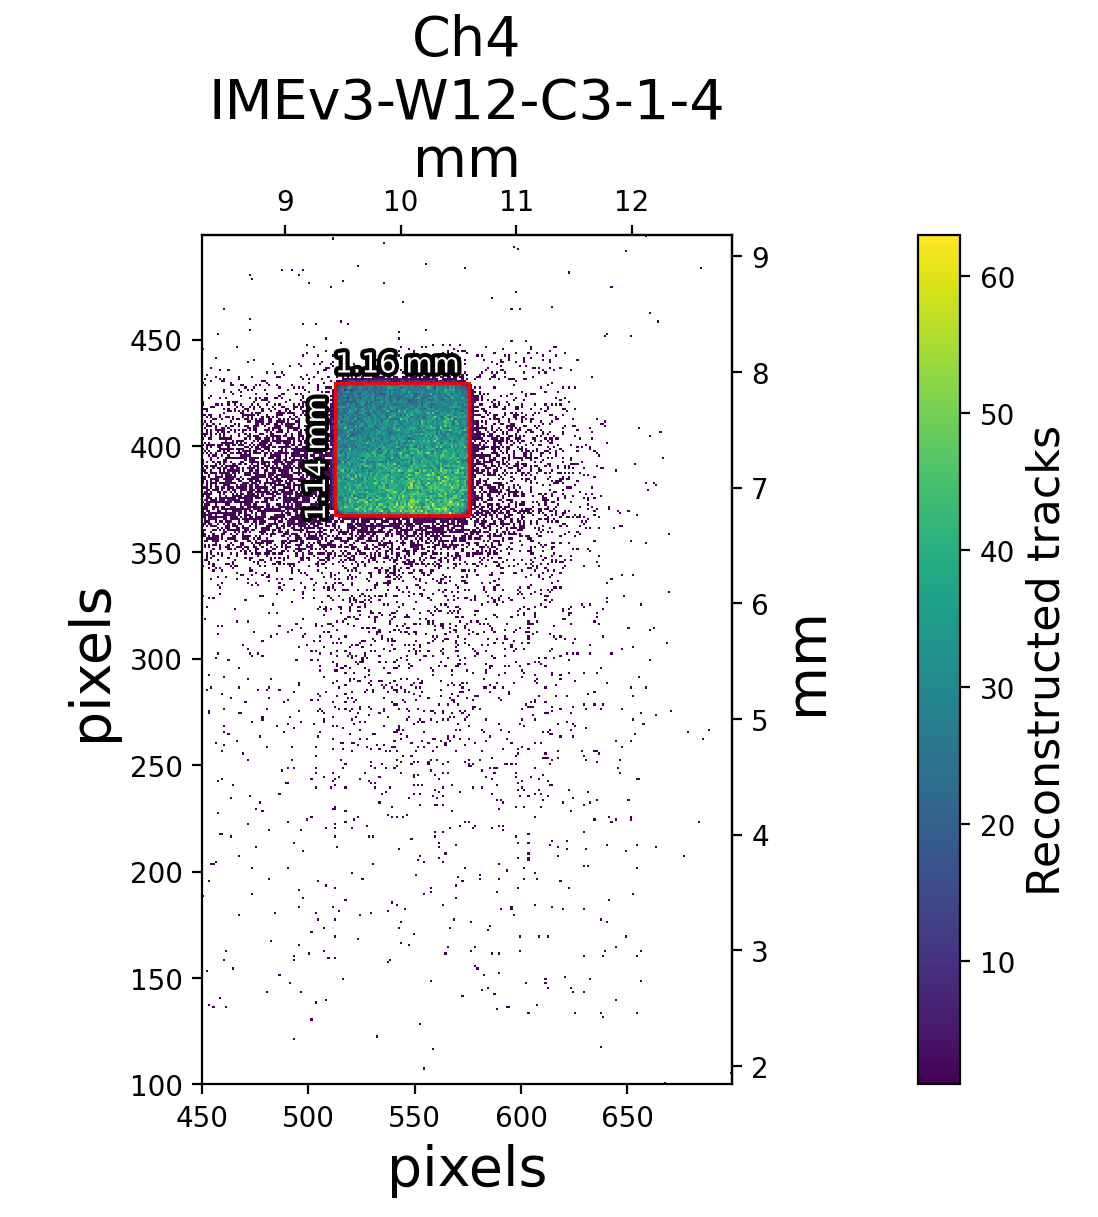
\includegraphics[width=.47\linewidth]{Images/methods/2D_Tracks_401_S1 highlight geometry cut (using pulseHeight).png}
        \label{fig:pulseHeight_cut_highlight}}
    \captionsetup{width=\captionwidth}
    \caption{The events selected by applying a pulse height cut}
\end{figure}

\subsection{Time cut}\label{subsec:time_cut}

The physical distance between the MCP and the DUT was fixed, and the momentum of the particles was constant throughout all the runs. Thus, the flight time of the particles between the MCP and the DUT was peaked around one point. Using this knowledge, an additional cut on the \(\Delta t\) was applied.

Firstly, the distribution of \(\Delta t\) (\(t_{DUT}-t_{MCP}\), time of arrival of the DUT - MCP) without any other cut was fit with a Gaussian plus a uniform background (Figure~\ref{fig:time_cut_gauss+bg_fit}):

\begin{figure}[h!tbp]
    \centering
    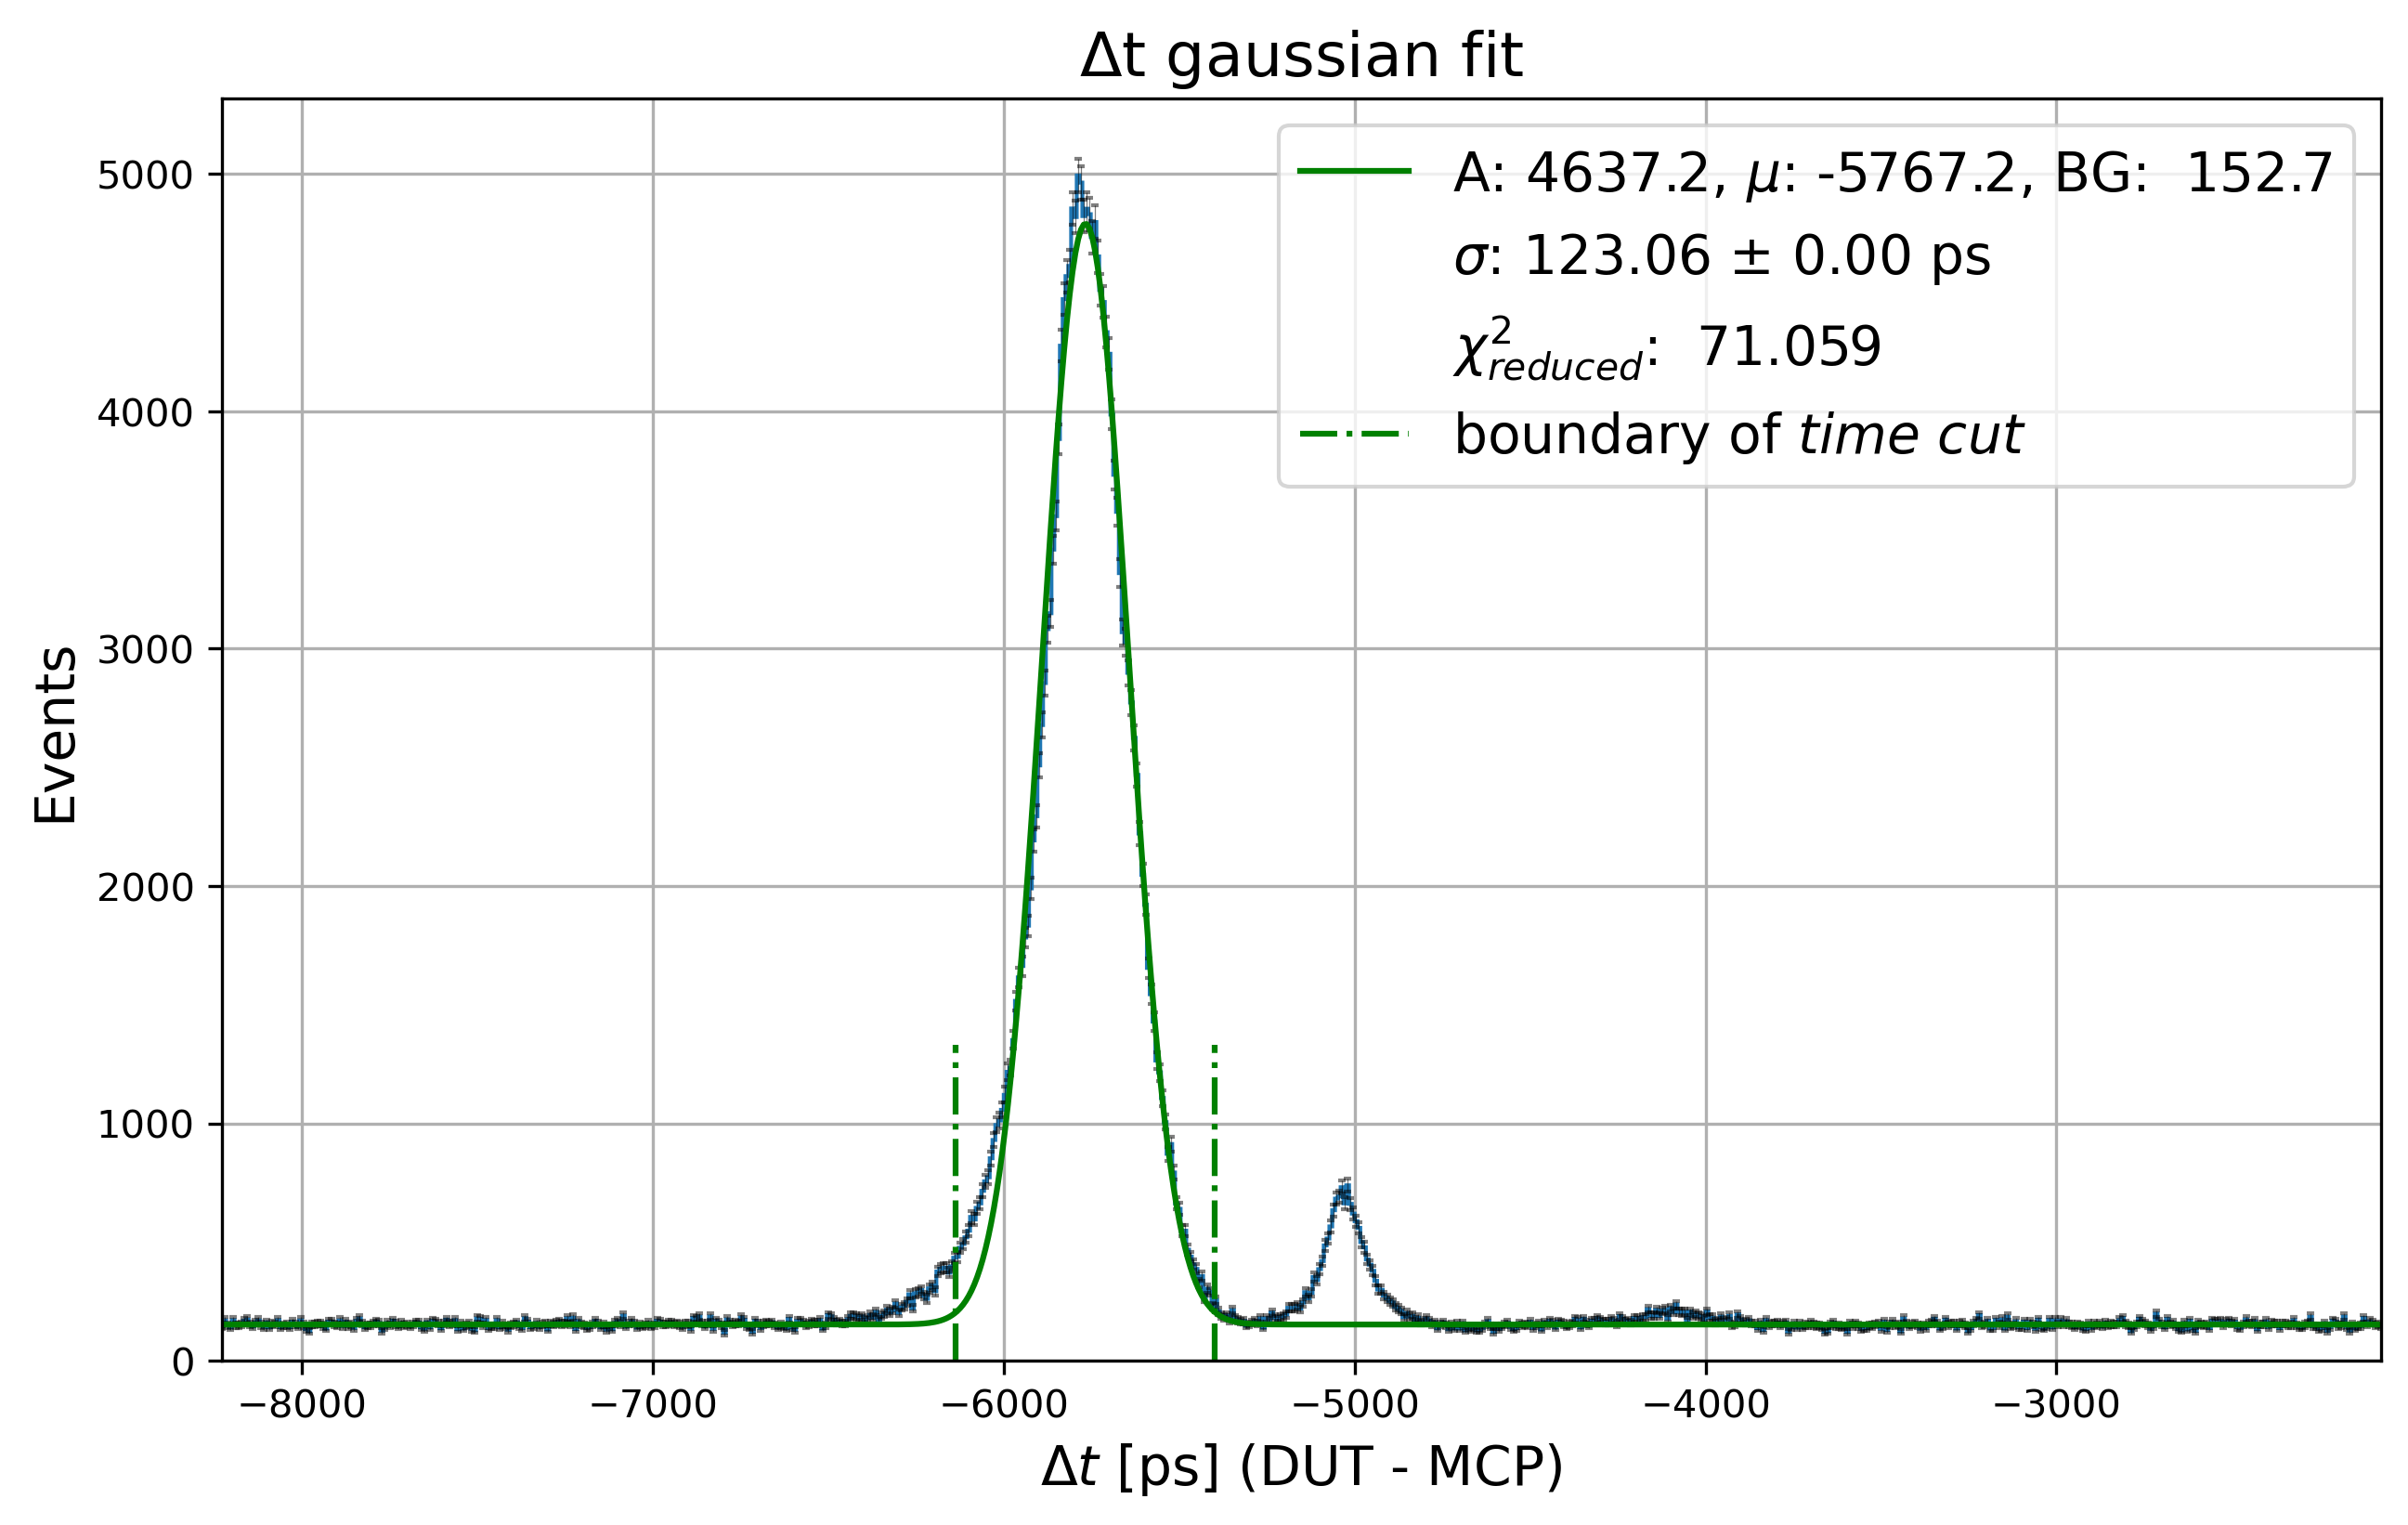
\includegraphics[width=.9\linewidth]{Images/methods/time_difference_603_S2_gauss_fit_no_cuts_DUT2.png}
    \captionsetup{width=\captionwidth}
    \caption{Time difference distribution (\(t_{DUT}-t_{MCP}\)) fit with a Gaussian + uniform background. The vertical dashed lines represent the boundary set as \textit{time cut}. The presence of the secondary peak is explained in Section~\ref{sec:multiple_peaks}.}
    \label{fig:time_cut_gauss+bg_fit}
\end{figure}

\begin{equation*}
    f(x,A,\mu,\sigma,BG) = A \cdot e^{-\frac{1}{2}\left(\frac{x-\mu}{\sigma} \right)^2} + BG  \, .
\end{equation*}

\(A:\) Amplitude (n° of events);\quad \(\mu:\) Mean of the gaussian;\quad \(\sigma:\) Standard deviation;\quad \(BG:\) Uniform BackGround.

Ultimately, a \textit{time cut} was defined as all the events lying inside an interval of a number \(n\) of standard deviations \(\sigma\):

\begin{equation}
    (\mu-n\sigma;\mu+n\sigma) \, .
\end{equation}

Given that roughly 99.7\% of all values of a normal distribution lie within 3 standard deviations, \(n=3\) was deemed an adequate choice.

This cut proved to be especially useful in calculating the total efficiency of each pad and in fitting the charge distribution.

Although, some peculiarities became apparent, namely the second peak shifted to the right of the main one (meaning delayed compared to the latter) and some discrepancy with the expected Gaussian distribution around the left tail. These effects were further investigated and will be explained later in Sections \ref{sec:multiple_peaks} and \ref{sec:deviations_from_gaussian}.

\subsubsection{Heavily radiated sensor case}\label{subsec:geometry_cut_w/pulse_cut}

In some cases, typically for heavily radiated sensors, the noise in the pulse height distribution was too large (Figure~\ref{fig:pulseHeight_cut_failed}) to allow a \textit{pulse height cut} as in Section~\ref{subsec:pulseHeight_cut}. This happened due to the pulse height decreasing and the noise peaks rising, so the separation between the two became less marked. In these situations it was possible to apply a \textit{time cut} instead and still get a satisfactory contour of the pad. The results of the two methods were very similar (Figure~\ref{fig:geometry_cut_comparison} in \nameref{chap:appendix}) so this seemed a good alternative.

\begin{figure}[h!tbp]
    \centering
    \subfloat[Pulse height distribution, without a clear boundary between noise and signal. The orange belt represents the poissonian error.]{
        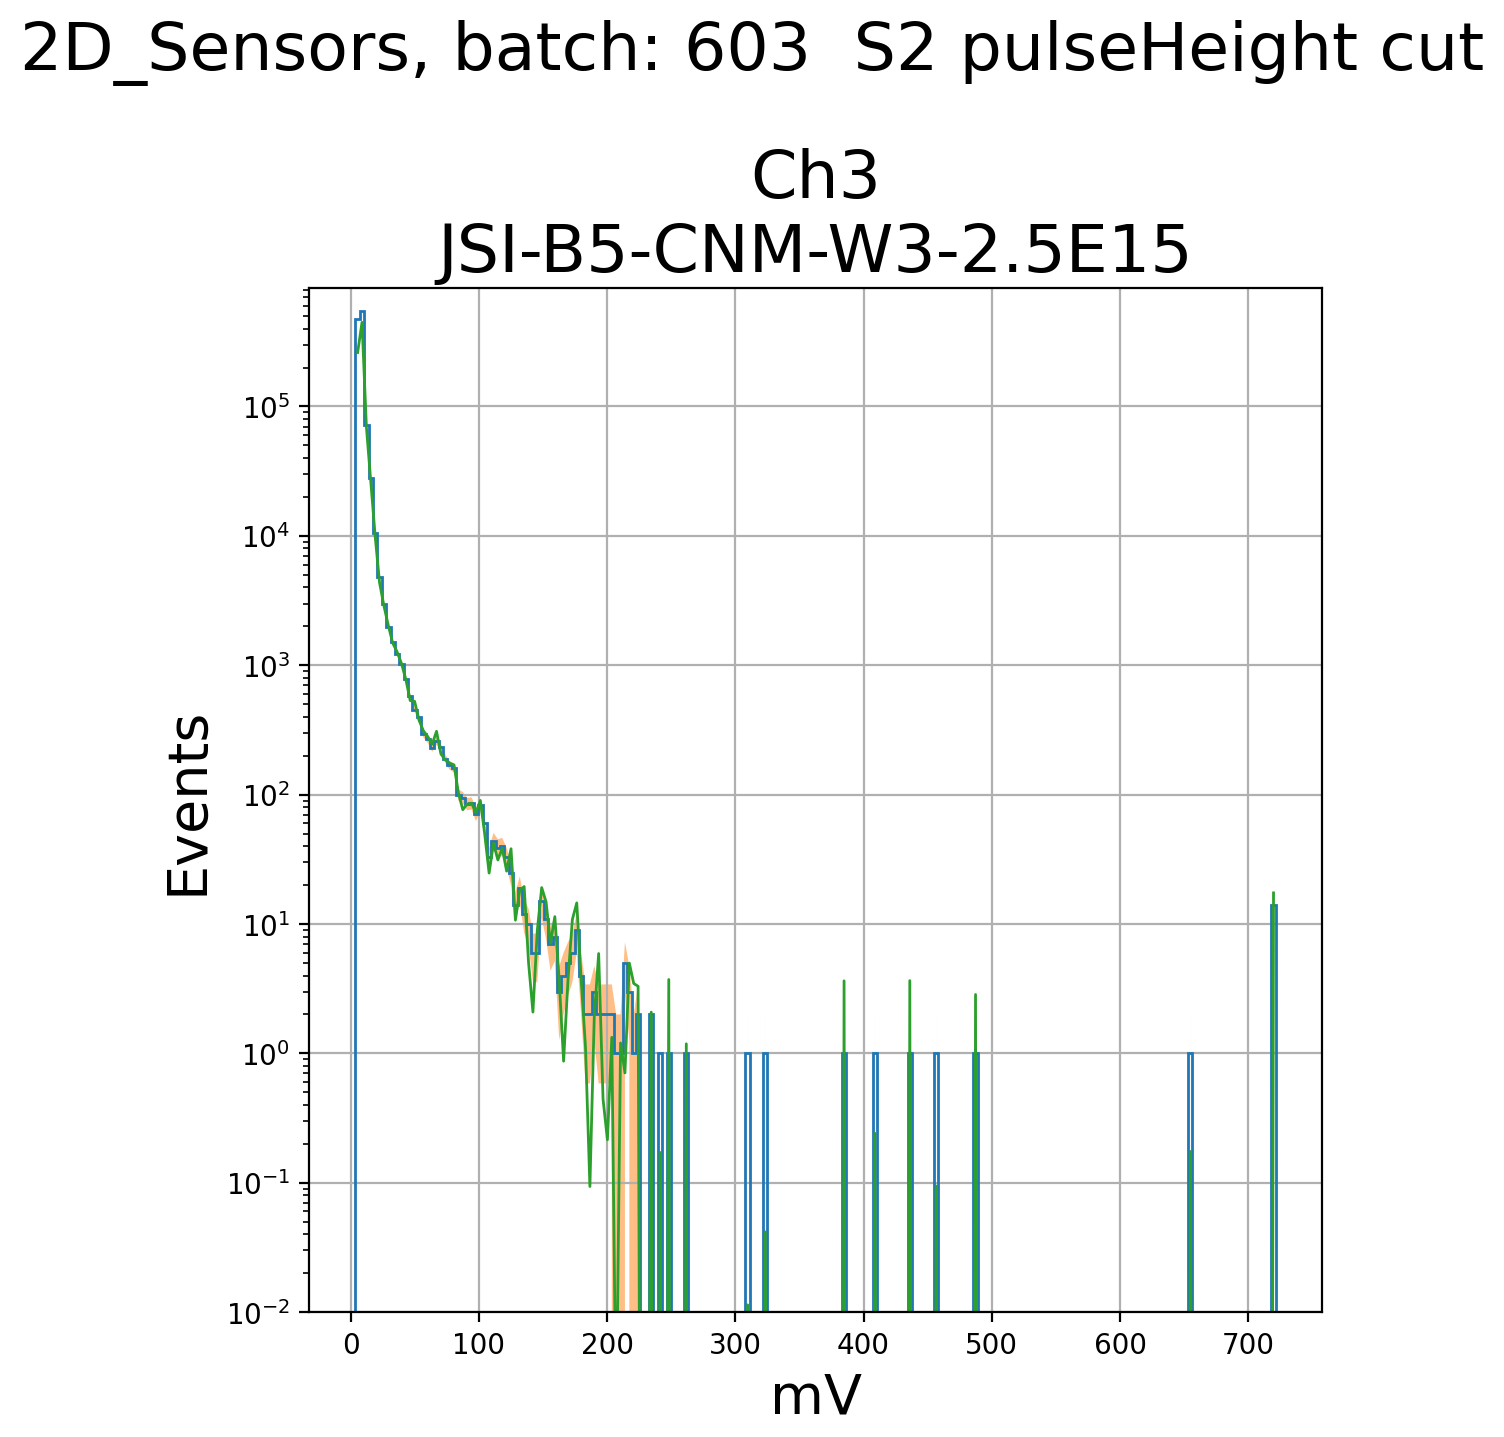
\includegraphics[width=.4\linewidth]{Images/methods/2D_Sensors_603 S2 pulseHeight cut_only_pulse.png}
        \label{fig:pulseHeight_cut_failed}}
    \hfill
    \centering
    \subfloat[Contour of the pad, highlighted in red, found by applying a time cut to the data. The irregular shape of the pad is caused by the ROI selected by the FEi4.]{
        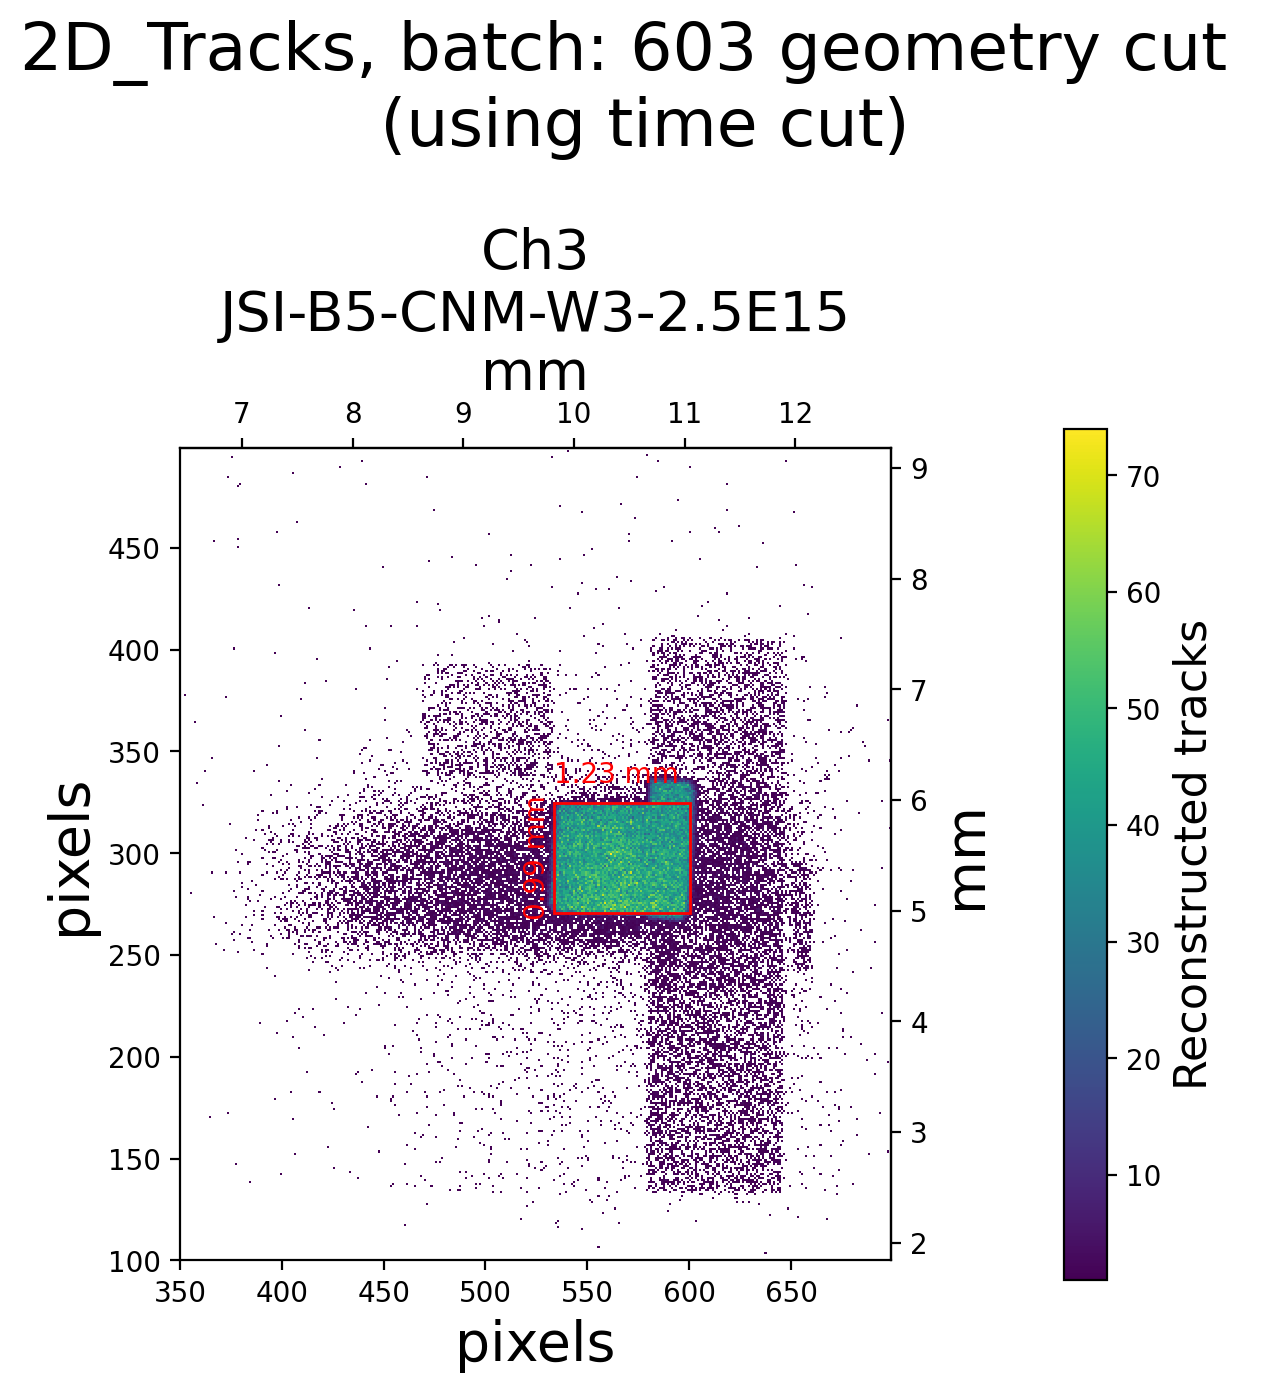
\includegraphics[width=.55\linewidth]{Images/methods/2D_Tracks_603_S2 highlight geometry cut (using time).png}
        \label{fig:time_cut_highlight}}
    \captionsetup{width=\captionwidth}
    \caption{Example of a different sensor (irradiated), for which the previous \textit{pulse height cut} became impractical (left), but using \textit{time cut} yielded a reasonable outline of the pad (right)}
\end{figure}

\subsection{Quality cuts validation}

To qualitatively confirm the soundness of the cuts performed, we plotted the density distribution of events of \(\boldsymbol{\Delta t}\) vs \textbf{pulse height} (Figures~\ref{fig:time_pulseHeight_nocut} and \ref{fig:time_pulseHeight_center}). The left plot shows all the available tracks, the right plot shows only the tracks that pass through the smaller central area of the DUT (a square of \(0.5\times0.5\unit{\milli\meter^2}\) explained in Section~\ref{sec:geometry_cut}).

The narrow selection of events in the right plot is very likely to be real signals (as they are particles guaranteed to have passed through the sensor). By comparing it with the plot on the left it can be noticed that a horizontal cut (\nameref{subsec:pulseHeight_cut}) and two vertical cuts (\nameref{subsec:time_cut}) provide indeed a good filter for physically meaningful events. 


\begin{figure}[h!tbp]
    \centering
    \subfloat[Density plot of all the events without any cuts applied.]{
        \includegraphics[width=.47\linewidth]{Images/methods/Time_pulseHeight_401S1_DUTs_3_(3,).png}
        \label{fig:time_pulseHeight_nocut}}
    \hfill
    \centering
    \subfloat[Density plot selecting only tracks passing through the central \(0.5\times0.5\unit{\milli\meter^2}\) area of the pad.]{
        \includegraphics[width=.47\linewidth]{Images/methods/Time_pulseHeight_401S1 central area_DUTs_3_(3,).png}
        \label{fig:time_pulseHeight_center}}
    \captionsetup{width=\captionwidth}
        \caption{Density plot of events when no cuts are applied (left) and when only a central square in the sensor is selected (right). The comparison between the two plots validated our choices made for quality cuts.}
\end{figure}


\section{Collected charge}\label{sec:methods_collected_charge}

A central goal of this study was to measure the distribution of the charge collected by the pads and verify their correspondence with the theoretical distribution: a convolution of a Gaussian and a Landau distribution (Appendix \ref{sec:vavilov_vs_landau_distribution}).

To achieve this, all the quality cuts defined in Section~\ref{sec:qualtiy_cuts} were applied, and a fit was carried out using an implementation of the Gaussian*Landau convolution provided by the ROOT framework~\cite{Brun:1997pa} (Figure~\ref{fig:charge_ROOT_fit}).

The collected charge of a sensor is defined as the most probable value (MPV) of the charge, i.e. the highest point in the distribution.

\begin{figure}[h!tbp]
    \centering
    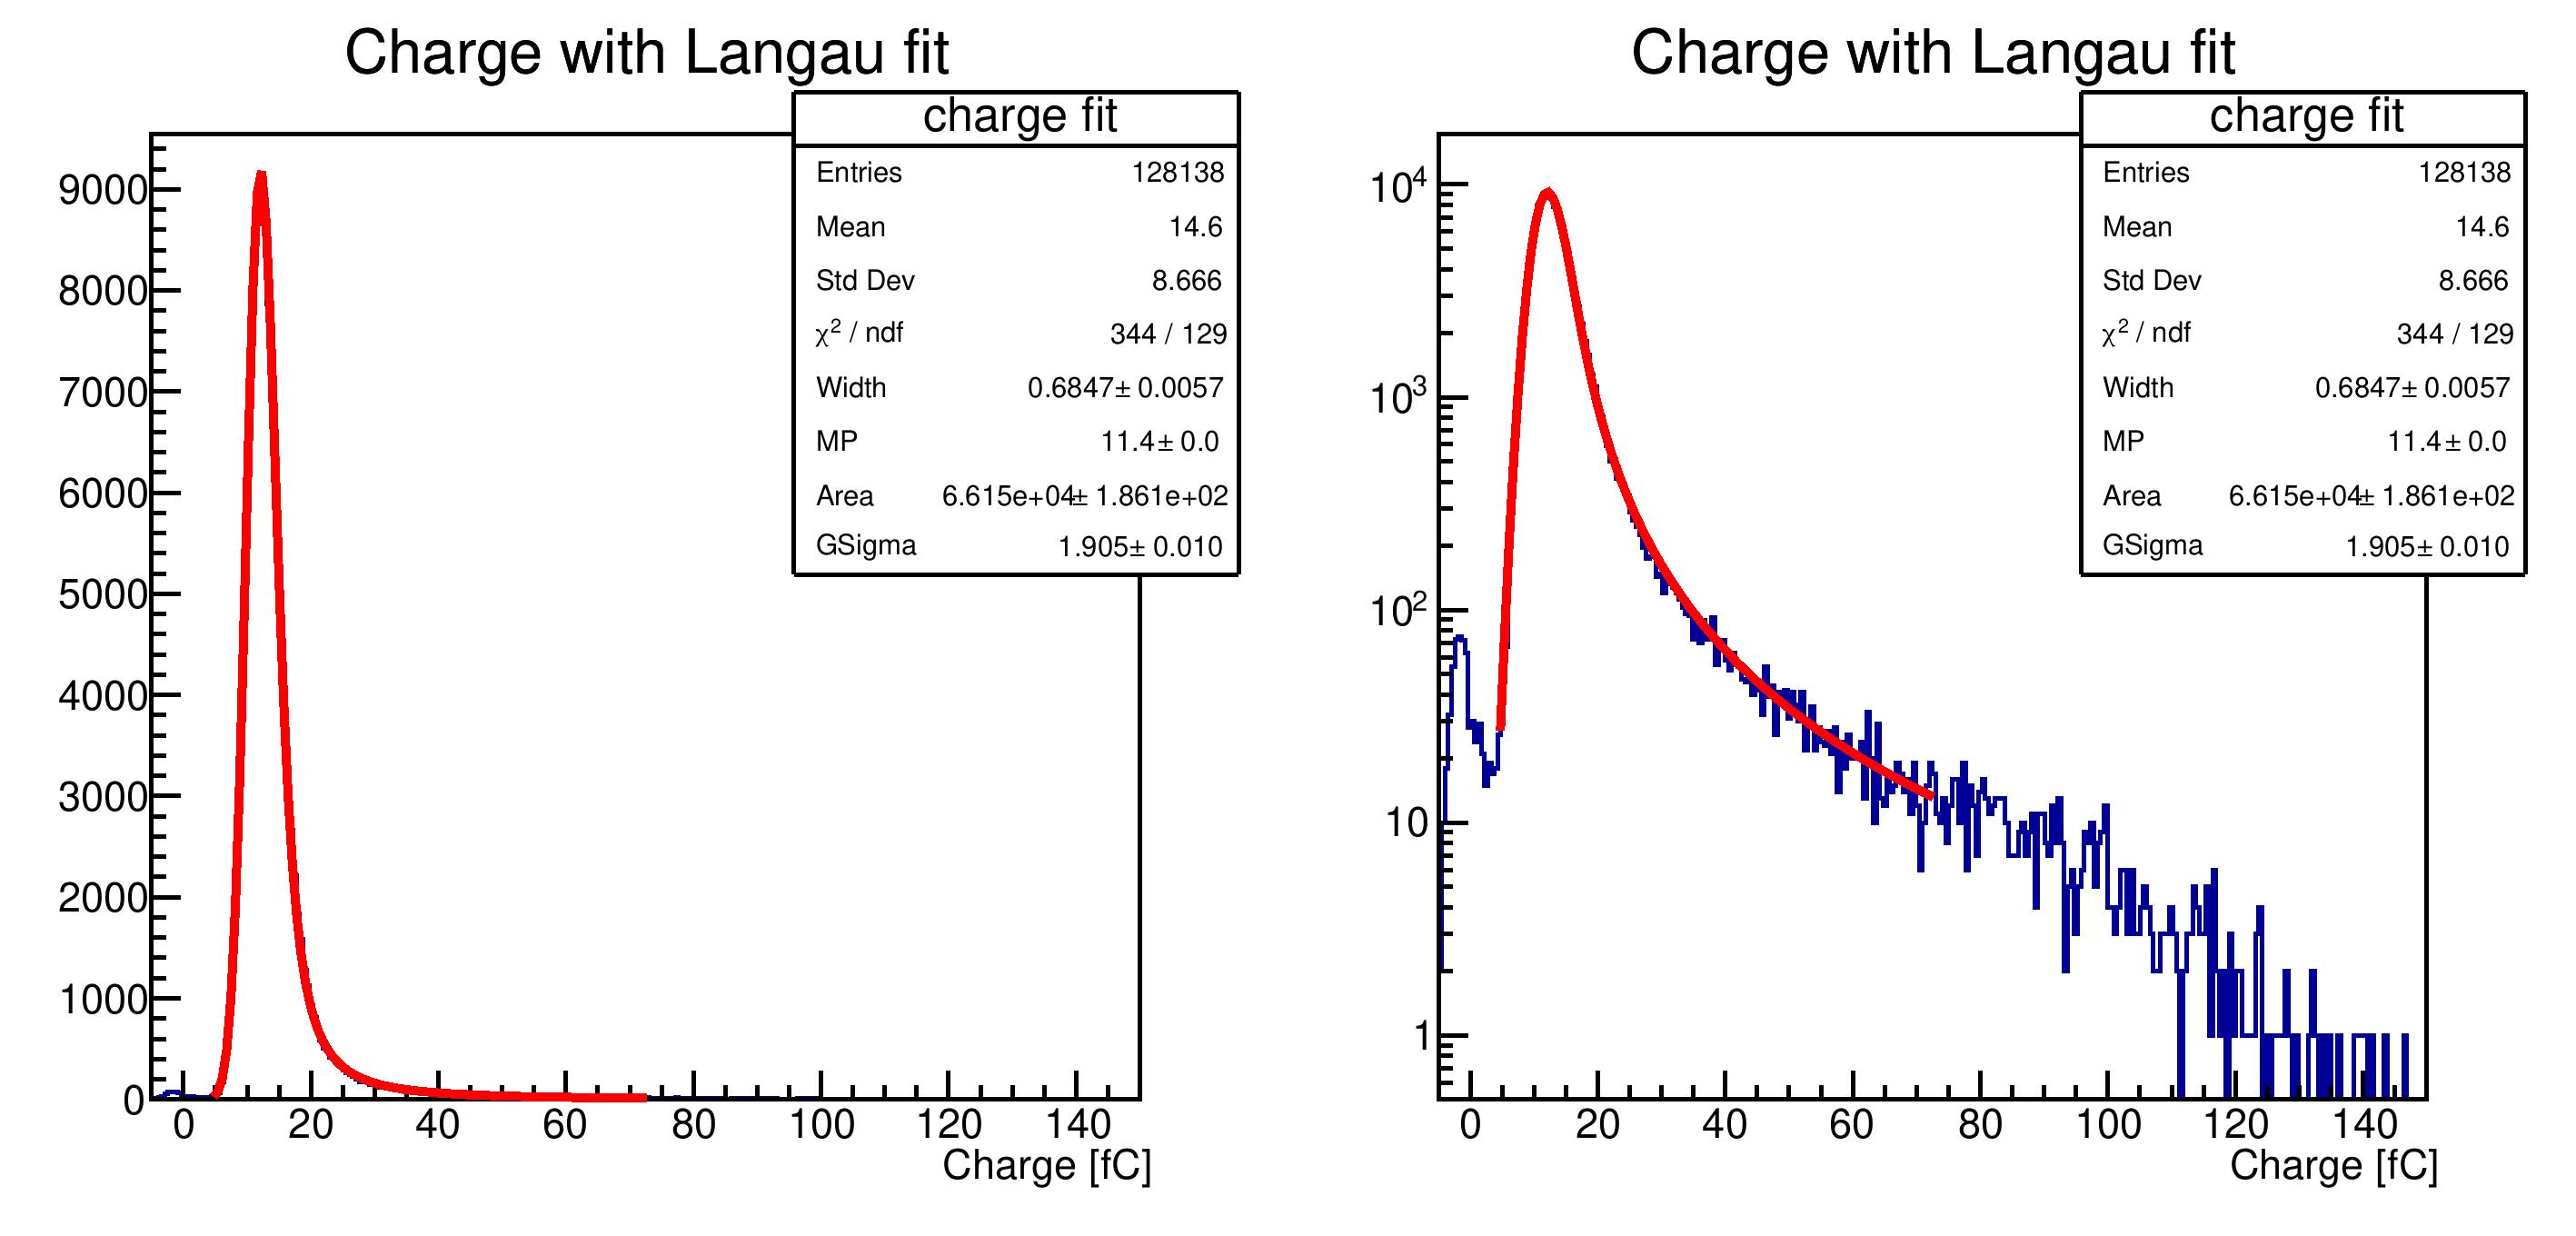
\includegraphics[width=1\linewidth]{Images/methods/charge_data_all_cuts_401_S1_3_Charge_fit_ROOT_double_plot.png}
    \captionsetup{width=\captionwidth}
    \caption{Fit of the charge distribution (red) carried out with ROOT. On the right it is shown the same plot in logarithmic scale, to highlight the extra noise at \(\approx 0\).}
    \label{fig:charge_ROOT_fit}
\end{figure}

\subsubsection{Gain}
% charged particle in 50 um of silicon produce ~0.52 fC of charge or 3280 e-h pairs
The gain is obtained by dividing the most probable value of the collected charge by the expected charge from a minimum ionizing particle (MIP) in a silicon sensor without gain. For a \qty{50}{\micro\meter} thick sensor, this value is \(3280\) e-h pairs, equivalent to \qty{.52}{\femto\coulomb} \cite{meroli_energy_loss2011}.

\subsubsection{Extra noise}
Despite all the trimming to the data, a noticeable part of the noise centered at \(\approx 0\) could not be removed. We could not pinpoint the origin of this extra noise, but a lot of factors could contribute to it: track reconstruction, other electronic noise etc.
Considering this point, the fit was performed in a smaller interval, avoiding the noise (Figure~\ref{fig:charge_ROOT_fit}). The left limit was fixed at \(4\si{fC}\), as this is also the lowest signal that the electronic board is able to measure, the right limit was adjusted to include only bins with significant amount of data (and account for the \nameref{subsec:charge_irregularities}, described in Appendix).

%%% maybe I can put a table to show which cuts I applied to which variables


\section{Efficiency}\label{sec:methods_efficiency}

The efficiency (\(\epsilon\)) was defined as the total number of tracks with charge larger than a certain \textit{threshold charge} divided by the total number of reconstructed track (\textbf{after} quality cuts had been applied).

% \begin{equation*}
%     \text{Efficiency} = \frac{\text{Tracks with } q>Q_{threshold}}{\text{Total tracks}}  \, .
% \end{equation*}

\begin{equation*}
    \epsilon = \frac{\text{Tracks with } q>Q_{threshold}}{\text{Total tracks}}  \, .
\end{equation*}

The threshold charge \(Q_{threshold}\) was chosen to be \(4\si{fC}\), which corresponds to the limit of sensitivity of the ASIC.

Before measuring the overall efficiency of the sensors, we applied a \textit{time cut} (as described in \nameref{subsec:time_cut}). Additionally, we elected to restrict the calculation to the smaller \textit{central area} of \(0.5\times0.5\unit{\milli\meter^2}\) defined earlier in Section~\ref{sec:geometry_cut}. This area can be seen highlighted in red in Figure~\ref{fig:efficiency_2D_plot}, which also shows the efficiency value computed for each individual squared binning of the surface.

Finally, the total efficiency was also computed with different values of \textit{threshold charge} to obtain the plot in Figure~\ref{fig:efficiency_depending_threshold}, which shows that (in this example) the value remains constant well after the chosen threshold of \(4\si{fC}\).

\begin{figure}[h!tbp]
    \centering
    \includegraphics[width=0.7\linewidth]{Images/methods/efficiency_plots/2D Efficiency_401_S1_with_time_cut_with_center_highlight_DUTs_3.png}
    \captionsetup{width=\captionwidth}
    \caption{2D histogram plot of the efficiency (per squared bin) and the \textit{central area cut} highlighted in red.}
    \label{fig:efficiency_2D_plot}
\end{figure}

\begin{figure}[h!tbp]
    \centering
    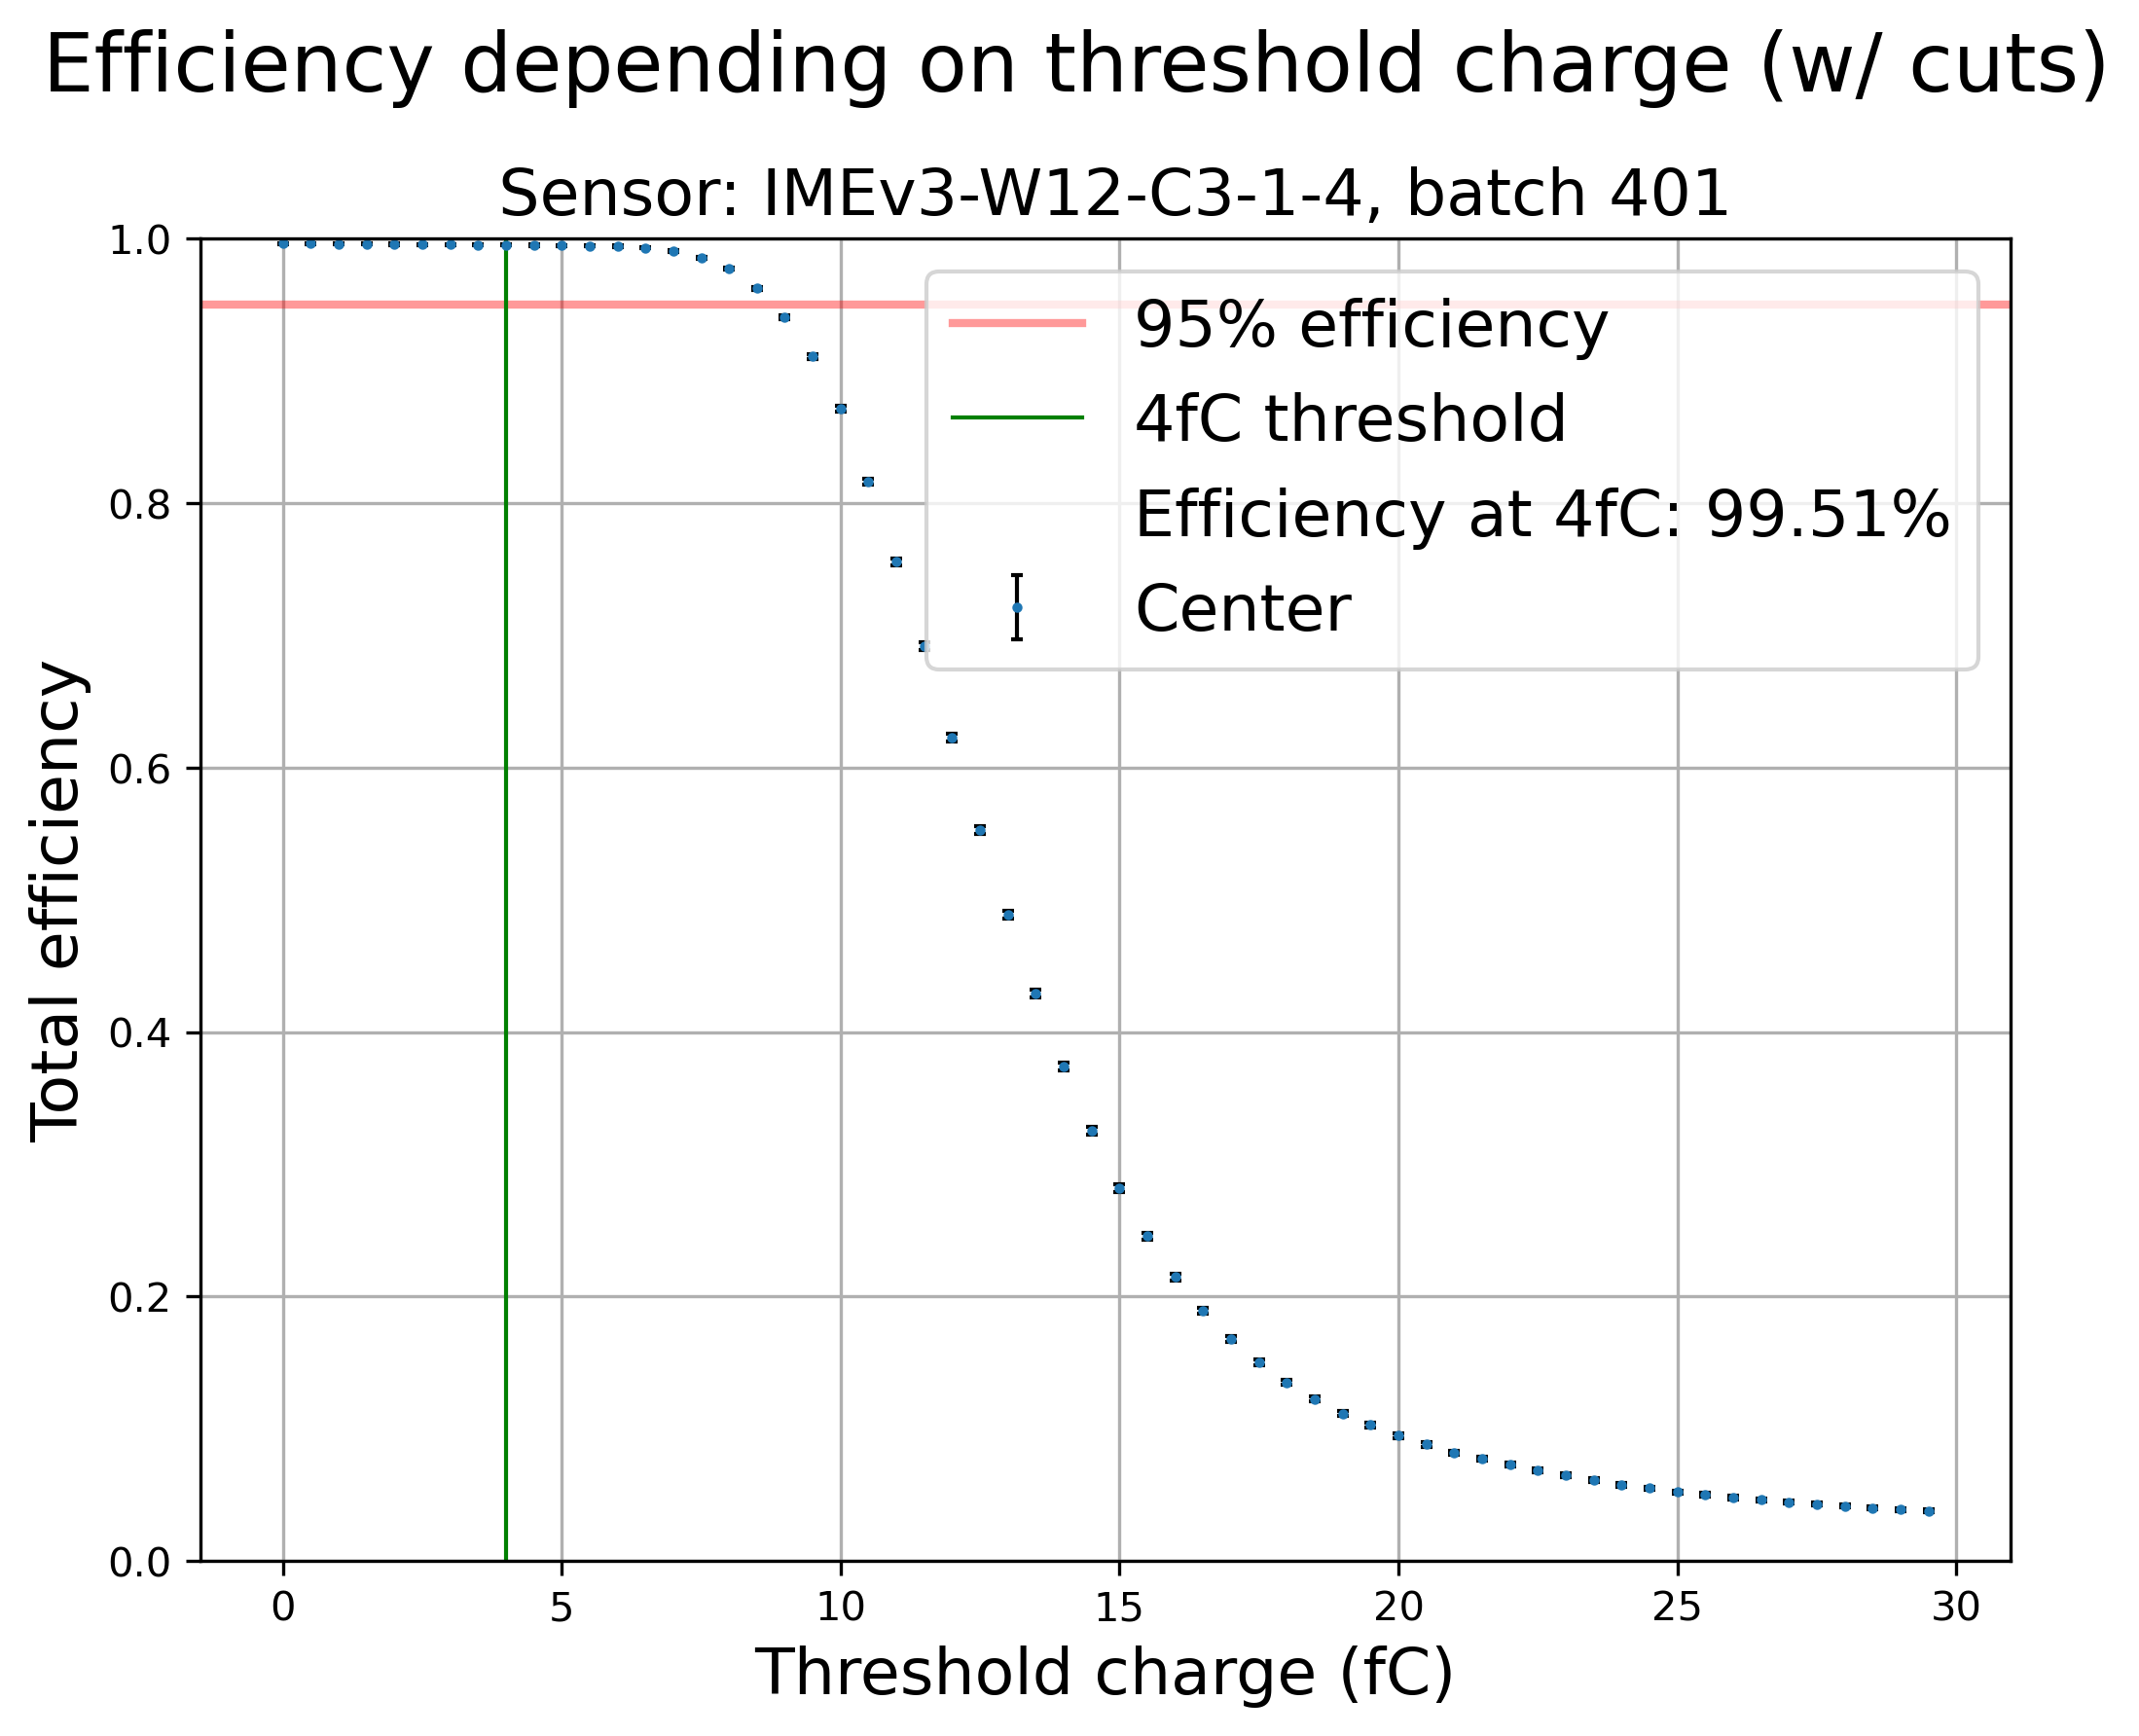
\includegraphics[width=0.5\linewidth]{Images/methods/efficiency_plots/Efficiency depending on threshold charge (with cuts) batch 401 S1.png}
    \captionsetup{width=\captionwidth}
    \caption{Total efficiency when changing the threshold value, ensuring that there is a large plateau of high efficiency.}
    \label{fig:efficiency_depending_threshold}
\end{figure}


\section{Time Resolution}\label{sec:methods_time_resolution}

The difference of times of arrival between the DUT and the MCP was fitted with a normal distribution. The standard deviation of said distribution corresponded to the time resolution of the DUT and MCP combined. Using simple error propagation, the time resolution of the DUT was computed: 

\begin{equation*}
    \begin{gathered}
    \sigma_{dut+MCP} = \sigma_{dut} \oplus \sigma_{MCP} \\
    \downarrow \\
    \sigma_{dut+MCP}^2 = \sigma_{dut}^2 + \sigma_{MCP}^2 \\
    \sigma_{dut} = \sqrt{\sigma_{dut+MCP}^2-\sigma_{MCP}^2}  \, .
    \end{gathered}
\end{equation*}


\begin{figure}[h!tbp]
    \centering
    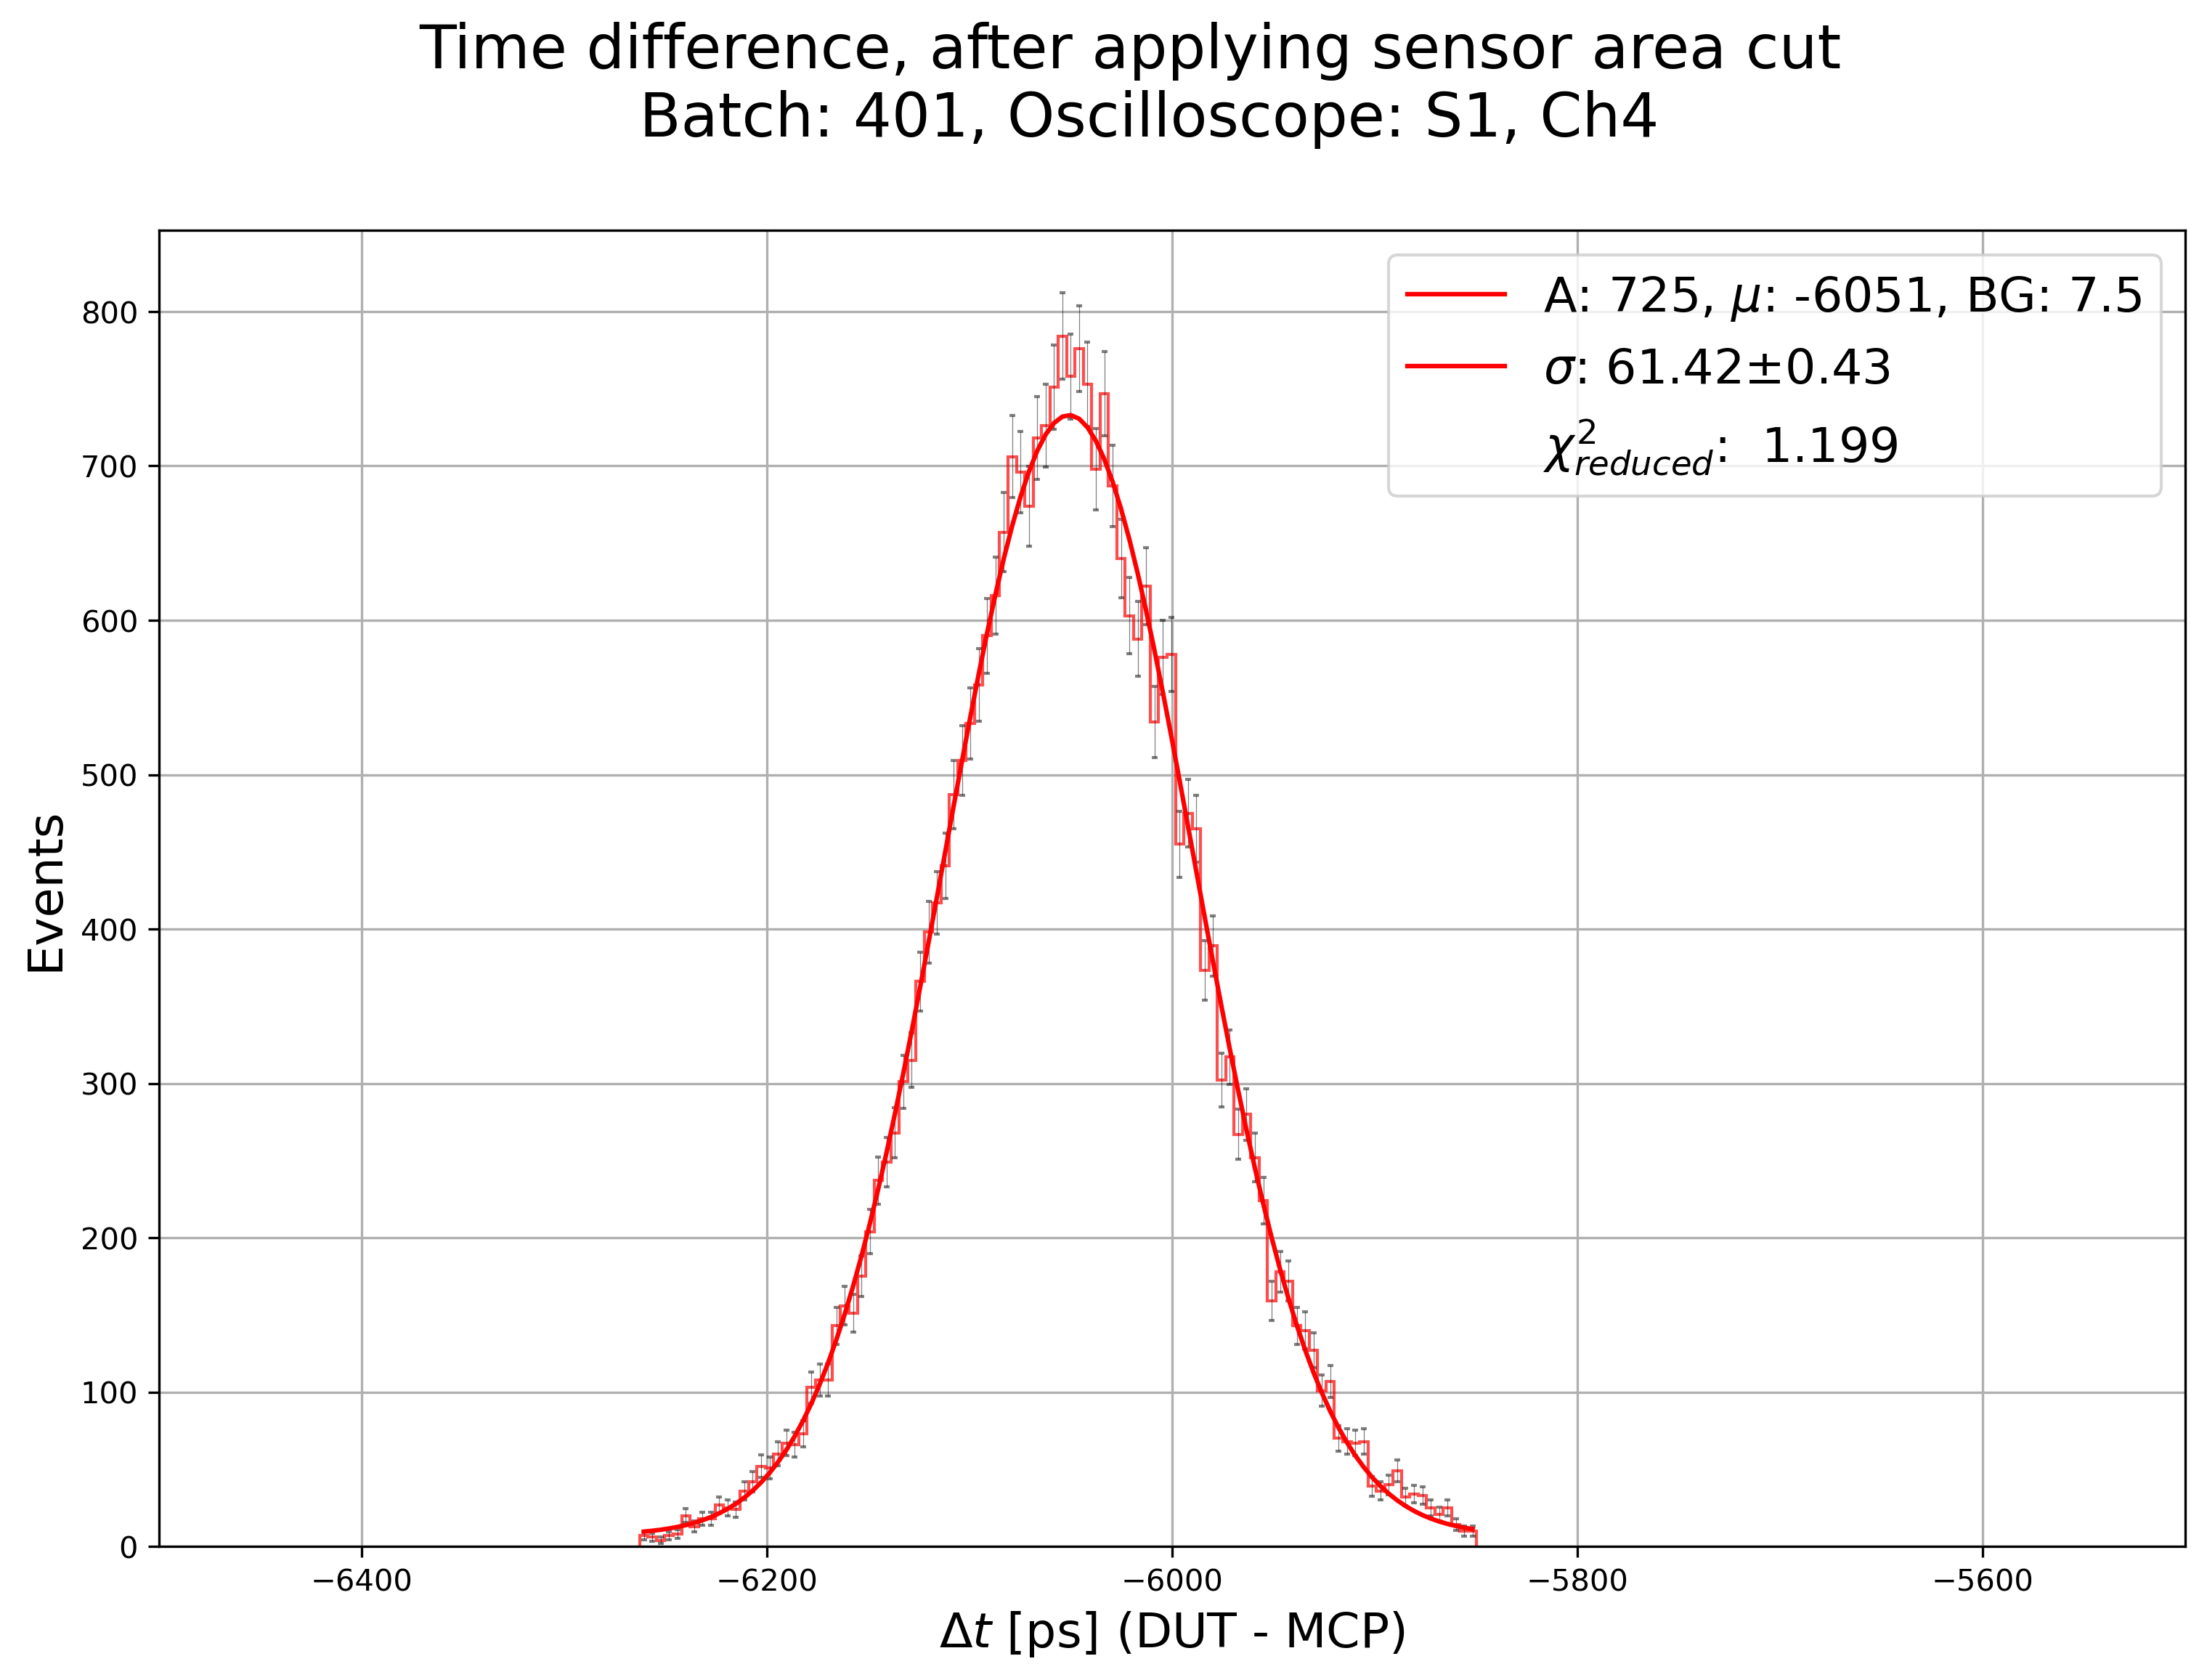
\includegraphics[width=0.7\linewidth]{Images/methods/time_resolution_plots/time_difference_401_S1_zoomed_and_gauss_fit_with_cuts_central_area_DUTs_3.png}
    \captionsetup{width=\captionwidth}
    \caption{Gaussian fit of \(\Delta t\) to find the time resolution (\(\sigma\)), the error bars are the statistical poissonian error (\(y_{err}=\sqrt{N}\)). For this sensor the final time resolution was \(\sigma_{dut} = 47.72\pm0.88\si{\ps} \).}
    \label{fig:time_resolution_plot}
\end{figure}


